\documentclass{article}
\usepackage{amsmath} 
\usepackage{graphicx}

\begin{document}
Auclert, Rognlie and Straub (2018) make the case that the iMPC, or Intertemporal MPC that measures how households respond at time $t$ to an income shock arriving at time $s$ is a crucial statistic for understanding both monetary and fiscal policy responses.

In particular they show the \textit{cumulative} fiscal multiplier, when prices are perfectly sticky and real interest rates fixed, is equal to one in most standard models (including TANK), but that it can become large in a model that more accurately matches empirical iMPCs.

Here I show in a particularly simple model of household behavior that the iMPCs cannot be used to determine cumulative fiscal multipliers, in the sense that iMPCs that are $\varepsilon$ different imply infinitely different cumulative multipliers.

Indeed, we will show that includes any patient households, cumulative multipliers must be equal to one.

We then compare the simple model we present to a fully micro-founded HANK model. We show which aspects of the HANK model it is able to well capture, which it misses, as well as ways in which it may be superior. If we can get empirical evidence on the shape of iMPCs from Scandanavia that would be amazing. My hunch is that they will look much more like the simple model presented below (with non-symetric responses to money arrival).

\section{Geo-RANK}
The Geo-RANK model (so called because it has geometric declining iMPCs) is a very simple model in which households spend a constant fraction of their market resources:
\begin{align*}
C_t = \alpha M_t \\
\end{align*}
The iMPCs are shown in figure \ref{fig:iMPC_RANK}. With $\alpha=0.25$ the quarterly MPC is 0.25 and the annual MPC is 0.68, approximately in line with the empirical evidence. In contrast to the HANK model in Auclert, Rognlie and Straub (2018), the later iMPCs are completely assymetric (households do not spend the money in anticipation).
\begin{figure} 
	\begin{centering}
		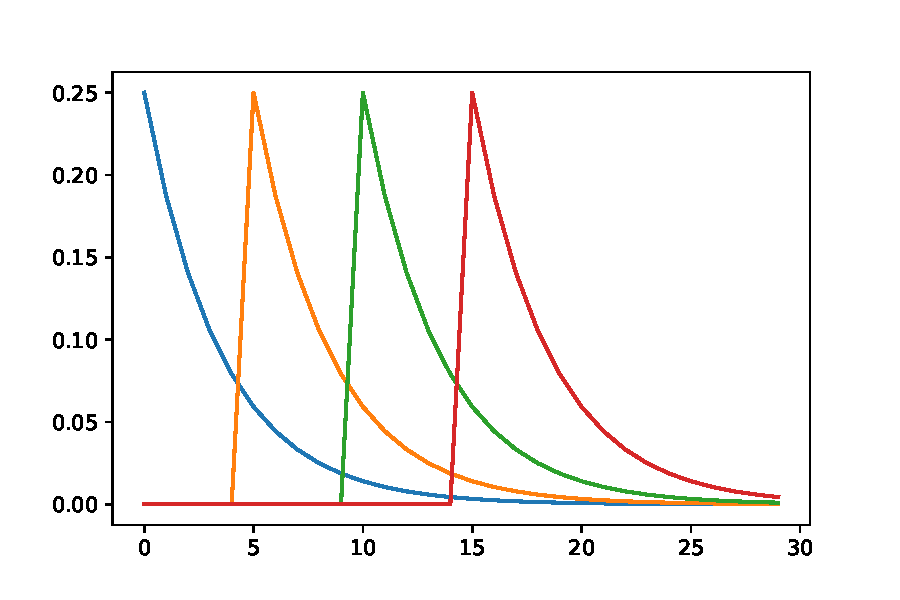
\includegraphics[scale=0.7]{../../Python/DoloCode/GeoTANK/Figures/iMPC_RANK.pdf}
		\caption{iMPCs in GeoRANK model with $\alpha=0.25$}
		\label{fig:iMPC_RANK}
	\end{centering}
\end{figure}
An economy made up of such agents, with prices completely sticky and real interest rate fixed, can be written down as:

Agent's decision rules:
\begin{align*}
C_t = \alpha M_t \\
M_t = Y_t + R A_{t-1} -T_t \\
A_t = M_t - C_t \\
\end{align*}
Aggregation equations:
\begin{align*}
Y_t = C_t + G_t \\
A_t - B =   \rho_B(A_{t-1} - B + G_t ) \\
G_t = \rho_G G_{t-1} + \varepsilon^G_t
\end{align*}
Where $A_t$ are end-of-period savings, $G_t$ government expenditures and $B$ steady state government debt. $\rho_G$ is the rate of decay of a government spending shock, initially we will set this at zero. $\rho_B$ is the rate at which the government debt is repaid.

The impulse response functions are shown in figure \ref{fig:GeoRANK_irf}
\begin{figure} 
	\begin{centering}
		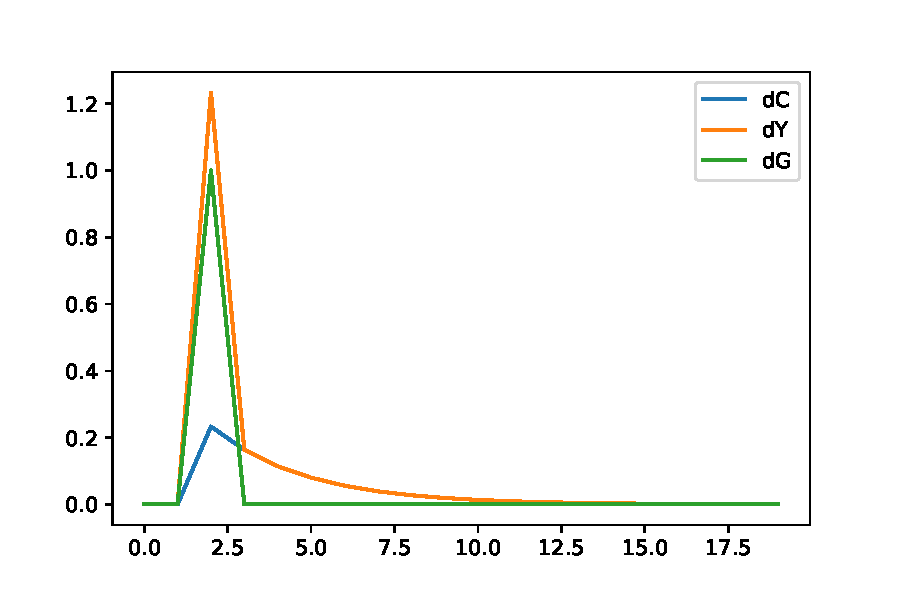
\includegraphics[scale=0.7]{../../Python/DoloCode/GeoTANK/Figures/GeoRANK_irf.pdf}
		\caption{Impulse response GeoRANK model with $\alpha=0.25$ and $\rho_B=0.7$}
		\label{fig:GeoRANK_irf}
	\end{centering}
\end{figure}
The impact multiplier is 1.23 and the cumulative multiplier is 1.76



\section{Geo-TANK}
The Geo-TANK model extends the model above to add some fraction of unconstrained, forward looking, rational agents. The idea is very similar to a standard TANK model, but instead of hand-to-mouth agents, we have agents who behave as in the Geo-RANK model. The introduction of even a fraction $\varepsilon$ of these agents qualitatively changes the model. In fact, in this model cumulative multipliers are exactly equal to one.

Here is the model (written in changes from steady state):

First equations for the Geo-agent
\begin{align*}
dC^g_t = \alpha M^g_t \\
dM^g_t =d Y_t + R d A^g_{t-1} -T_t \\
dA^g_t =d M^g_t -d C^g_t \\
\end{align*}
Next equations for the rational agent (note as long as we return to steady state, these equations imply $dC^r_t=0$ for all $t$. The rational agents do not change their consumption at all, as long as interest rates remain constant.
\begin{align*}
dC^r_t = dC^r_{t+1} \\
dM^r_t =d Y_t + R d A^r_{t-1} -T_t \\
dA^r_t =d M^r_t -d C^r_t \\
\end{align*}
Finally aggregation equations. We set a fraction $\lambda$ of Geo-agents
\begin{align*}
dY_t = dC_t + dG_t \\
dA_t = \lambda dA^g_t + (1-\lambda)dA^r_t \\
dC_t = \lambda dC^g_t + (1-\lambda)dC^r_t
dG_t = \rho_G dG_{t-1} + \varepsilon^G_t \\
dA_t = \rho_B (dA_{t-1} + dG_t)
\end{align*}

The impulse response functions are shown in figure \ref{fig:GeoTANK_irf}
\begin{figure} 
	\begin{centering}
		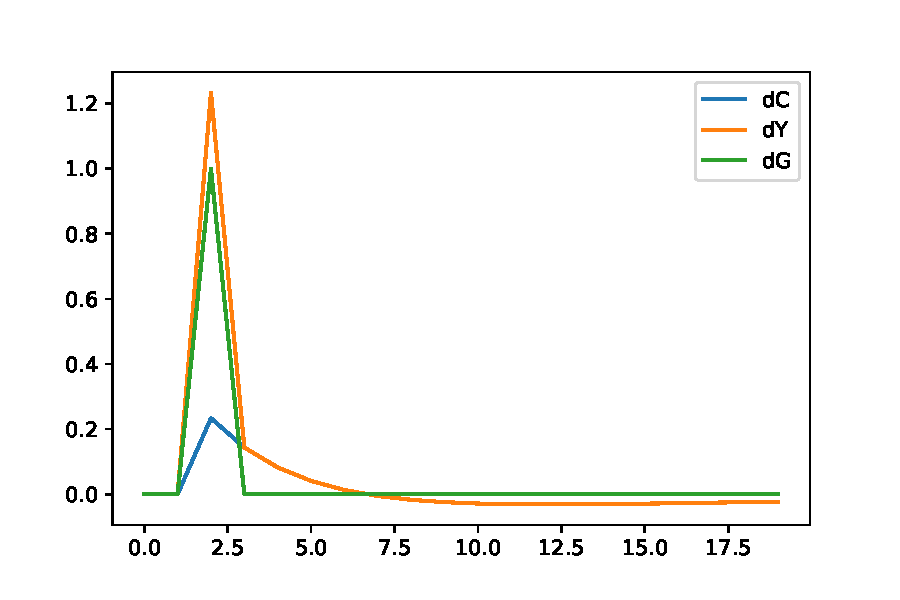
\includegraphics[scale=0.7]{../../Python/DoloCode/GeoTANK/Figures/GeoTANK_irf.pdf}
		\caption{Impulse response GeoTANK model}
		\label{fig:GeoTANK_irf}
	\end{centering}
\end{figure}
Here I have set $\lambda=0.8$ and $\alpha= 1 - \frac{\lambda-\alpha}{\lambda}$ so that the first period MPC matches $\alpha$, that in the GeoRANK model. Note that the impact multiplier is now exactly the same, 1.23, but the cumulative multiplier is now exactly one. After seven quarters, consumption turns negative and then slowly assymptotes back to zero.

The top panel of figure\ref{fig:multipliers} shows the impact multipliers for the two models are identical, and increasing linearly in $\rho_B$, the speed at which the government pays back debt. Compare this to Figure 4 in Auclert, Rognlie and Straub (2018) for which the HA-illiquid model begins to curve up as $\rho_B$ increases. The difference is due to the (slightly) forward looking nature of agents in the HA-illiquid model, so the slower debt repayments in the next few periods lead to more consumption today.
\begin{figure} 
	\begin{centering}
		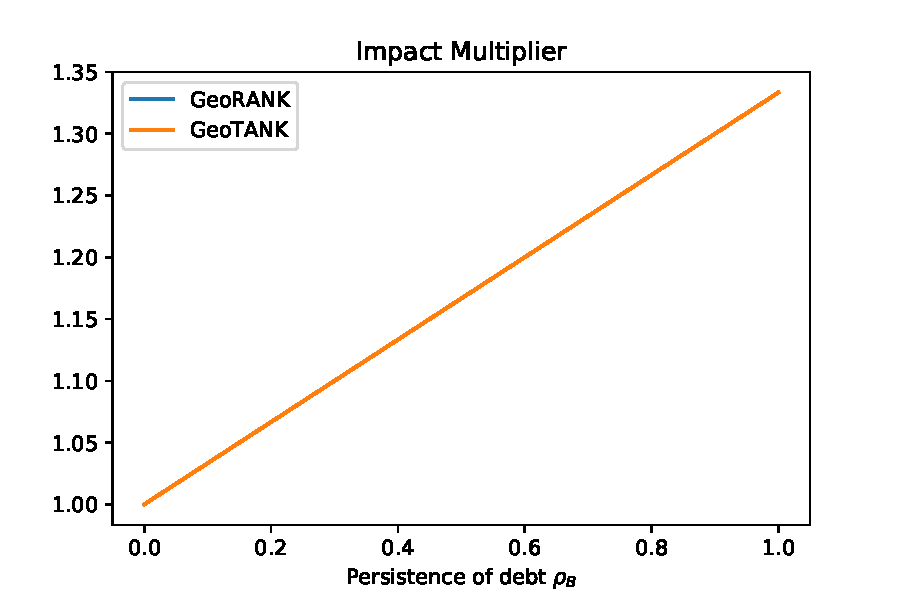
\includegraphics[scale=0.6]{../../Python/DoloCode/GeoTANK/Figures/impact_multiplier.pdf}		
		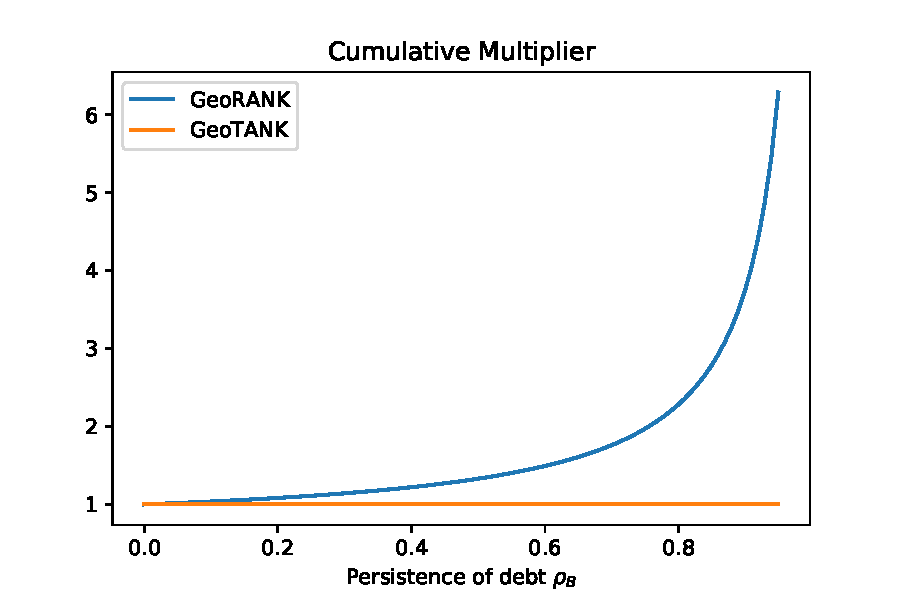
\includegraphics[scale=0.6]{../../Python/DoloCode/GeoTANK/Figures/cum_multiplier.pdf}
		\caption{Impact and Cumulative multipliers in the GeoRANK and GeoTANK models}
		\label{fig:multipliers}
	\end{centering}
\end{figure}
The bottom panel shows the GeoRANK model behaves like the HA-illiquid model in figure 4 of  Auclert, Rognlie and Straub (2018), but as discussed the cumulative multiplier for the GeoTANK model is fixed at one.

The result will be more general - we could reproduce the HA-illiquid model and show the cumulative multipliers can be large. We could then add in some patient agents (either of the same type, but just with higher $\beta$, or totally unconstrained with $\beta=1/R$. We will show that the cumulative multipliers fall to very close to zero (or exactly zero in the case where we add some unconstrained agents.

Why is this? If the model has an agent who is unconstrained and has $\beta=1/R$,  then this agent must have $C_t = C_{t+1}$. If the model returns to steay state, this means this agent will not react at all to the fiscal policy shock. But if there was a cumulative multiplier greater than one, their intertemporal budget constraint would then not add up, so in equilibrium the cumulative multiplier in a model with ANY agents of this type must be equal to one.

What causes the discontinuity? In the GeoRANK model, the Geo agents have to hold on the all the government debt. In the GeoTANK model, the Geo agents spend faster than the rational agents, so the Geo agent bond holdings go down while the rational agent bond holdings go up. This slight 'leakage' of bonds from the Geo agents to the rational agents in the GeoTANK model results in convergence in the response to a one off increase in bonds that are never paid back, which is exactly offset by the taxes. Without this leakage, the two sums do not separately converge, so together can add up to something other than one.

\section{Hump shaped responses to Fiscal and Monetary Policy}

The results above about cumulative multipliers are not about the asymmetry of the Geo agent's iMPCs - they should hold in a HANK model as well (and we should show that).

What we do get from the asymmetry is humped shaped responses monetary and fiscal policy. This is a result that I think could be of a lot of interest.

The previous IRFs were drawn with a one off shock to government spending $(\rho_G=0)$. I now set a positive $\rho_G=0.5$, along with a relatively slow rate of debt repayment, $\rho_B=0.95$. The impulse response for the GeoRANK model is seen in figure \ref{fig:hump_fiscal}.

\begin{figure} 
	\begin{centering}
		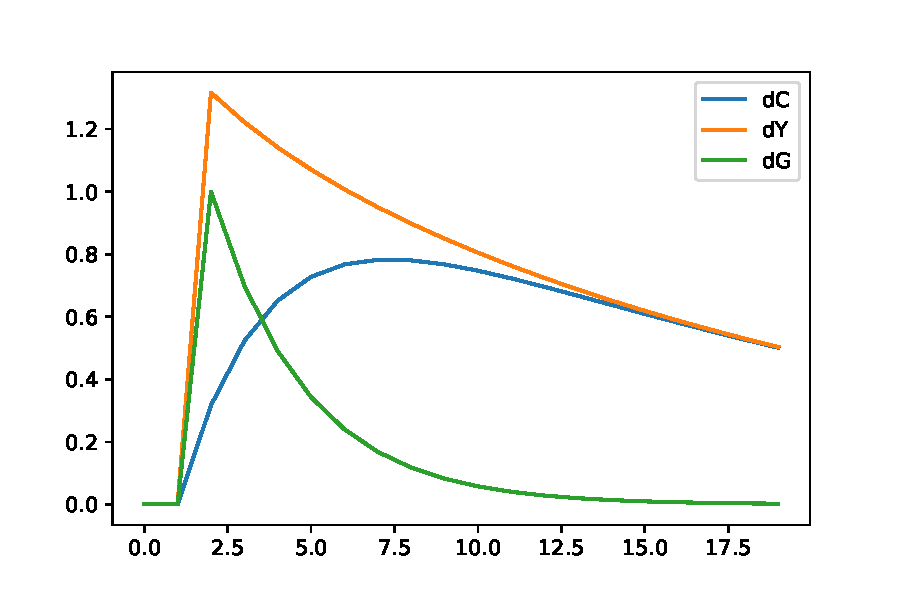
\includegraphics[scale=0.6]{../../Python/DoloCode/GeoTANK/Figures/GeoRANK_rho07_irf.pdf}		
		\caption{Humped Consumption Consumption Response in GeoRANK model}
		\label{fig:hump_fiscal}
	\end{centering}
\end{figure}

The peak consumption is reached at around 8 quarters after the initial shock, in line with some of the VAR literature.

We could do a similar exercise with monetary policy (in the GeoTANK model). With a negative shock to R, going back to steady state as AR(1), consumption of the Ricardian agents would be the same as usual, jumping at t=0 and slowly returning to zero. However, the Geo agents would see a hump shape to their consumption, leading overall to a somewhat humped shape.

If monetary policy acts through redistribution, this hump shape is even more pronounced. In this case, the Ricardian agents don't change their consumption much at all on the shock, but there is a flow of cash towards the Geo agents, who will build up their consumption slowly.

This would be further affected is households hold longer term debt, see figure \ref{fig:delayed_response}.

\begin{figure} 
	\begin{centering}
		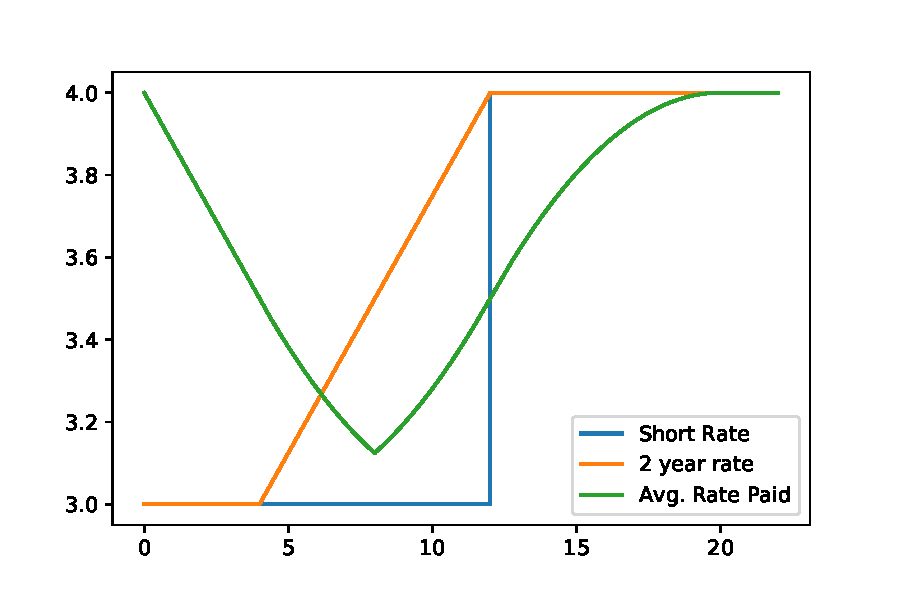
\includegraphics[scale=0.6]{../../Python/DoloCode/Figures/delayed_response.pdf}		
		\caption{Delayed response to a rate change for the actual rate being paid by households}
		\label{fig:delayed_response}
	\end{centering}
\end{figure}

\section{Empirical evidence of Asymmetric iMPCs?}

We will need some empirical evidence of asymmetric iMPCs for this to really get traction. Where can we find this?

Best: Norwegian spending data at a monthly (weekly?) frequency. Look at events such a bonus payments (perhaps know somewhat in advance), lottery winnings, tax rebates, inheritances. Also spending patterns around promotions - is there a delayed build up to new permanent spending rate?

CEX data - what evidence is there for the month before tax rebates? How does it compare with the month after?

Japanese data - my colleague possibly has some access

Is it symmetrical with downs as well as ups?


\section{Micro foundations for Asymmetric iMPCs?}
Can we micro found this in some way?

\end{document}